\section{Does a better initialization affect the final estimation?}
The standard initialization is to take $\mathbf{w}_0$ as the off-diagonal elements of the
pseudoinverse of the sample covariance matrix, denoted as $\hat{\boldsymbol{\Theta}}_{\textsf{scm}}$.
This is tantamount to solving the following problem
$$\begin{array}{ll}
  \underset{\mathbf{w}}{\textsf{minimize}} & ||\hat{\boldsymbol{\Theta}}_{\textsf{scm}} - \mathcal{L}\mathbf{w}||^{2}_{\text{off}, F}\\
  \textsf{subject to} & \mathbf{w} \geq \mathbf{0}.
\end{array}$$

In order to improve the initial estimate, we consider the following optimization problem
\begin{equation}
\begin{array}{ll}
  \underset{\mathbf{w}}{\textsf{minimize}} & ||\hat{\boldsymbol{\Theta}}_{\textsf{scm}} - \mathcal{L}\mathbf{w}||^{2}_{F}\\
  \textsf{subject to} & \mathbf{w} \geq \mathbf{0}.
\end{array}
\end{equation}
Note that,
\begin{equation}
||\hat{\boldsymbol{\Theta}}_{\textsf{scm}} - \mathcal{L}\mathbf{w}||^{2}_{F} =
||\text{vec}\left(\hat{\boldsymbol{\Theta}}_{\textsf{scm}}\right) - \text{vec}(\mathcal{L}\mathbf{w})||^{2}_{2} =
||\text{vec}\left(\hat{\boldsymbol{\Theta}}_{\textsf{scm}}\right) - \mathbf{R}\mathbf{w}||^{2}_{2},
\end{equation}
where $\mathbf{R}\triangleq \text{vec}\circ \mathcal{L}$.

We denote the above algorithm as \textsf{LLQP}. Figure~\ref{fig:initial-guess} shows the performance of the
$\textsf{SGL}$ algorithm when initialized by \textsf{LLQP} and \textsf{ISCM}. This experiment indicates that
the \textsf{SGL} algorithm remains neutral to the different initilization procedures discussed here, even though
it is clear that the \textsf{LLQP} shows a far better performance than \textsf{ISCM}.

\begin{figure}[!htb]
    \centering
    \begin{subfigure}[b]{0.45\textwidth}
        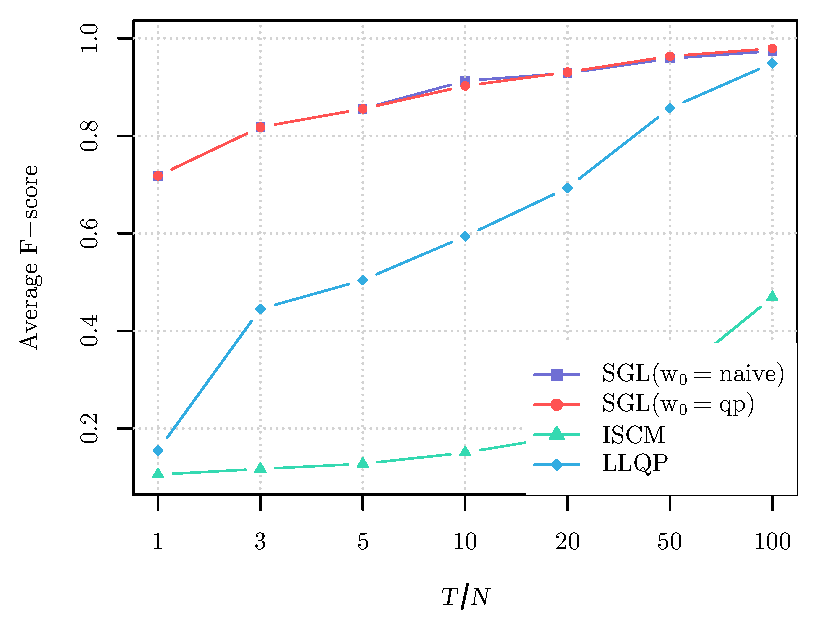
\includegraphics[width=\textwidth]{initial_guess/fscore.eps}
    \end{subfigure}
    ~ %add desired spacing between images, e. g. ~, \quad, \qquad, \hfill etc.
      %(or a blank line to force the subfigure onto a new line)
    \begin{subfigure}[b]{0.45\textwidth}
        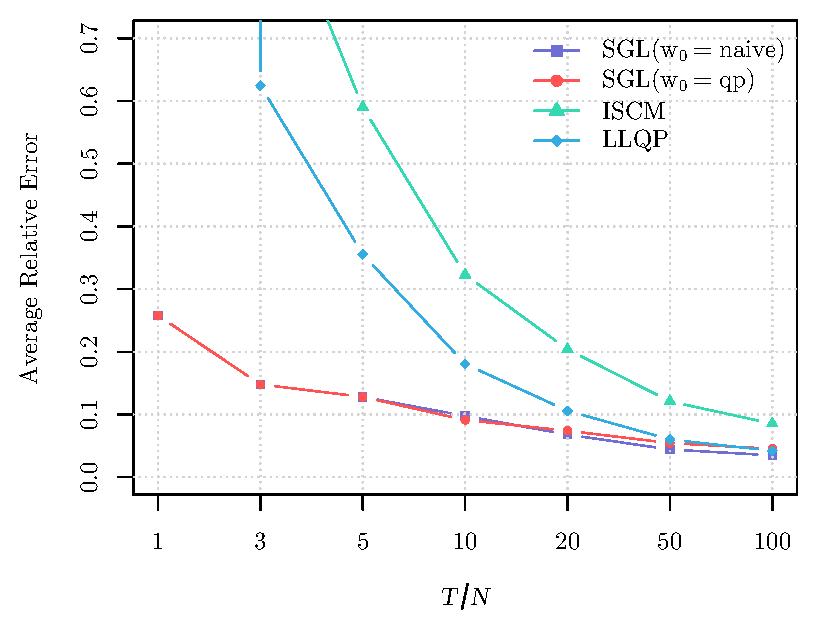
\includegraphics[width=\textwidth]{initial_guess/relative_error.eps}
    \end{subfigure}
    \caption{Relative error and F-score attained by \textsf{SGL} with different initialization strategies.
             \textsf{SGL}($\mathbf{w}_0 = \text{naive}$) and \textsf{SGL}($\mathbf{w}_0 = \text{qp}$)
           stand for the initialization with \textsf{ISCM} and \textsf{LLQP}, respectively.}
    \label{fig:initial-guess}
\end{figure}
